\documentclass{article}
\usepackage{graphicx} % Required for inserting images
\graphicspath{ {./images/} }
\usepackage{amsmath,amsthm,amssymb}
\usepackage{mathtext}
\usepackage[T1,T2A]{fontenc}
\usepackage[utf8]{inputenc}
\usepackage[english,russian]{babel}
\usepackage{multirow}

\DeclareMathOperator{\facmin}{facmin}
\DeclareMathOperator{\facmax}{facmax}
\DeclareMathOperator{\fac}{fac}
\DeclareMathOperator{\tol}{tol}
\DeclareMathOperator{\err}{err}
\title{отчет 2.47}
\author{nesterov.boris123 }
\date{December 2023}

\begin{document}



\section{Условие.}
Найти периодическое решение системы ДУ

$\left\{\begin{array}{l}\left\{\begin{array}{l}\frac{d x}{d t}=y, \\ \frac{d y}{d t}=\alpha\left(1-x^2\right) y-x,\end{array}\right. \\ \alpha \in\{0.1,10.0\} .\end{array}\right.$



\section{Решение.}
Система уравнений является частным случаем уравнения Ван-дер-Поля, записанного как система. Существование у этой системы предельного цикла и его единственность уже доказаны. Так же известно, что любое решение, не проходящее через критические точки будет сходиться к предельному циклу. Единственной критической точкой данного уравнения является $(0,0)$, так как из первого уравнения получаем $y = 0$, подставив это во 2 уравнение получим, что $x = 0$. Итак, если решение не начинается в $(0,0)$, оно будет сходиться к предельному циклу.

Будем рассматривать решение, начинающееся из точки $(1,0)$, и методом хорд искать точку его третьего пересечения прямой $y = 0$. Эти точки сходятся к точке предельного цикла, следовательно, можем взять достаточно близкую.

\section{Метод Рунге-Кутты.}
При решении был использован классический метод Рунге-Кутты 4 порядка


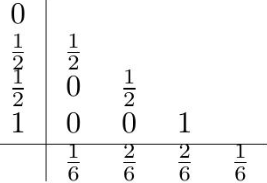
\includegraphics[width=0.4\textwidth]{rungeKutta}
Для определения ошибки на шаге делается один просчет с удвоенной длинной шага и 2 просчета с обычной (обозначим результаты $u_{2h}$ и $u_h$ соответственно). Далее, ошибка по каждой переменной считается по правилу Рунге с использовнием масштабирующего множителя.
Окончательная формула для подсчета ошибки выглядит следующим образом:
$$
d = \big|u_h + \frac{u_h - u_{2h}}{2^4-1}\big|
$$
$$
\err = \big| \frac{1}{2^4-1}\frac{u_h - u_{2h}}{d}\big|
$$
Затем, ошибкой на шаге принимается максимум из ошибок по каждой переменной.
\section{Выбор шага.}
Новый шаг рассчитывается по формуле $h_{\text {new }}=h \cdot \min(\facmax, \max(\facmin, \fac(\frac{\tol}{\err})^{(\frac{1}{p+1})})) $, где $p = 4, \facmax = 3, \facmin = 0.00001, \fac = 0.8$, а $\tol$ - это максимальная ошибка, при различных значениях которой делаются расчеты.

Если ошибка на шаге не превышает максимальной, полученное значение принимается, иначе производится пересчет с новым шагом.
\section{Результаты.}

Цикл при $\alpha = 0.1$

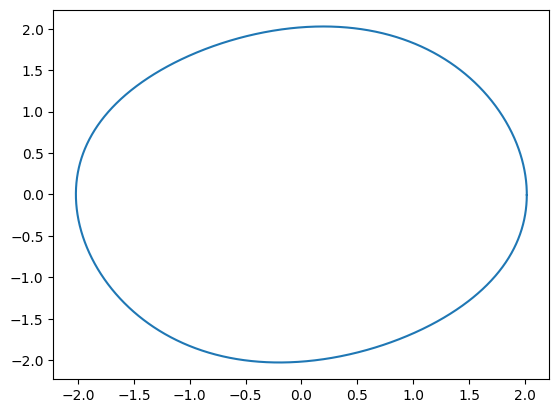
\includegraphics[width=0.7\textwidth]{alpha01}

Цикл при $\alpha = 10$

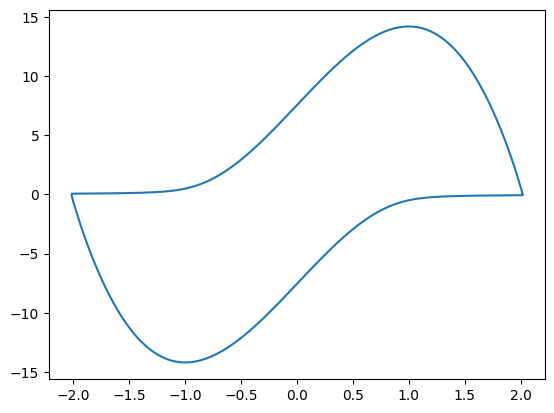
\includegraphics[width=0.7\textwidth]{alpha10}

В таблицах приведены результаты расчетов при различных значениях максимальной ошибки


\begin{tabular}{ |p{3cm}||p{3cm}|p{3cm}|  }
 \hline
 \multicolumn{3}{|c|}{$\alpha = 0.1$} \\
 \hline
 $\tol$ &Количество точек&Суммарная ошибка\\
 \hline
 $1e-7$& $118$ & $1.374860e-06$     \\
 $1e-9$& $280$ & $4.913808e-08$   \\
 $1e-11$ & $708$ & $1.166902e-09$\\

 \hline
\end{tabular}

\begin{tabular}{ |p{3cm}||p{3cm}|p{3cm}|  }
 \hline
 \multicolumn{3}{|c|}{$\alpha = 10$} \\
 \hline
 $\tol$ &Количество точек&Суммарная ошибка\\
 \hline
 $1e-7$& $1094$ & $1.828893e-05$     \\
 $1e-9$& $2744$ & $4.532883e-07$   \\
 $1e-11$ & $6892$ & $1.131785e-08$\\

 \hline
\end{tabular}


Для всех расчетов должно выполняться

$$
\frac{n_{i+2}}{n_{i}}=\left(\frac{\varepsilon_{i}}{\varepsilon_{i+2}}\right)^{1 / 5} \approx 2.5119, \quad \frac{e r r_{i}}{e r r_{i+2}}=\left(\frac{\varepsilon_{i}}{\varepsilon_{i+2}}\right)^{4 / 5} \approx 39.8107
$$

$\alpha = 0.1$

$\frac{n_9}{n_7} = 2.372$

$\frac{n_{11}}{n_9} = 2.528$

$\frac{errSum_7}{errSum_9} = 27.979$

$\frac{errSum_9}{errSum_{11}} = 42.109$


$\alpha = 10$

$\frac{n_9}{n_7} = 2.508$

$\frac{n_{11}}{n_9} = 2.512$

$\frac{errSum_7}{errSum_9} = 40.347$

$\frac{errSum_9}{errSum_{11}} = 40.0507$
\section{Оценка глобальной ошибки.}
Для оценки глобальной ошибки была использована следующая формула:
$$
\delta\left(x_{i+1}\right)=r_i+\delta\left(x_i\right) \cdot \exp \left(L_i\right),
$$
в которой $L_i$ было оценено максимум нормы матрицы Якоби на отрезке $\big((x_i,y_i),(x_{i+1},y_{i+1})\big),$ умноженный на длину этого отрезка, которую обозначим за $d_i$. В качестве нормы матрицы была выбрана логарифмическая норма, так как она приводила к меньшей оценке.
Матрица Якоби системы имеет следующий вид:
$$A = \begin{pmatrix}0 & 1\\
-\left( 2 \alpha x y\right) -1 & \alpha \, \left( 1-{{x}^{2}}\right) \end{pmatrix}.$$
Для того, чтобы найти ее логарифмическую норму, необходимо найти максимальное по модулю собственное значение матрицы
$$\frac{1}{2}\big(A + A^T\big) = \begin{pmatrix}0 & -\left( \alpha x y\right) \\
-\left( \alpha x y\right)  & \alpha \left( 1-{{x}^{2}}\right) \end{pmatrix}.$$
 Выше приведены графики логарифмической нормы матрицы Якоби для $\alpha = 0,1$ и $\alpha = 10$.
\begin{figure}
    \centering
    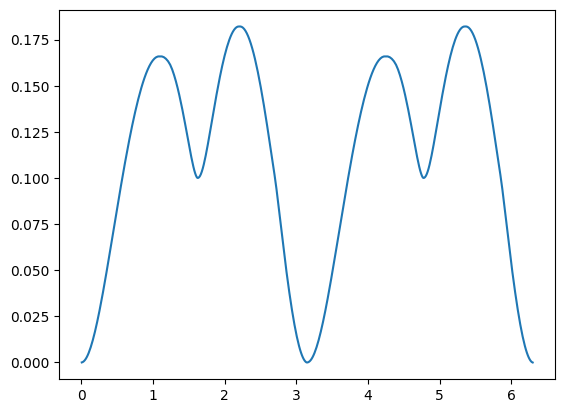
\includegraphics[width=0.5\linewidth]{images/image.png}
    \caption{$\alpha = 0.1$}
    \label{fig:enter-label}
\end{figure}
\begin{figure}
    \centering
    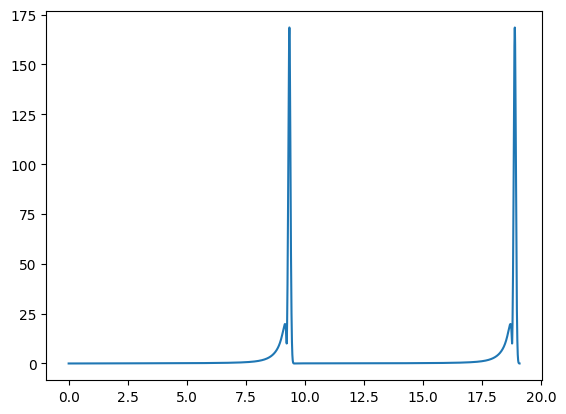
\includegraphics[width=0.5\linewidth]{images/log10.png}
    \caption{$\alpha = 10$}
    \label{fig:enter-label}
\end{figure}
Итоговая формула для расчета глобальной ошибки:
$$\delta\left(x_{i+1}\right)=r_i+\delta\left(x_i\right) \cdot \exp
\left(d_il_i\right)$$
$$l_i = \max\Big(\mu\big(A(x_i,y_i)\big),\mu\big(A(x_{i+1},y_{i+1})\big)\Big)$$
Значения оценки глобалбной ошибки приведены в таблице:
\begin{center}
  \begin{tabular}{|c|c|c|}
    \hline
    $\alpha$ & $\delta(x_N)$\\
    \hline
    $0.1$ & $1.709299e-09$\\
  \end{tabular}
\end{center}
\end{document}
